\chapter{Quantum Complexity}
Quantum complexity theory has been emerging as an important sub-field of quantum information theory, as it studies the hardness in solving computational problems, i.e. the resources needed for implementing the computation.
\\
Moreover, quantum complexity is recently being used as a measure of a certain distance between two quantum states. The usual metric in state space is the Fubini-Study metric, or the inner product metric. The Fubini-Study distance between two quantum states $\ket{A}$ and $\ket{B}$ ranges between 0 when the states are the same and $\frac{\pi}{2}$ when they are orthogonal. However, this distance misses an important aspect, which is the difficulty of the operation needed to go from $\ket{A}$ to $\ket{B}$. Quantum relative complexity, on the contrary, is able to capture this \cite{brown2018second}. It is defined for states as the size of the smallest circuit, which is a collection of gates, required to go from one state to another. Similarly, it is defined for unitaries as the least number of gates needed to go from one unitary to another.


\section{Evolution of quantum complexity}
The importance of quantum complexity makes it necessary to understand its growth and evolution with time. In \cite{brown2018second}, Brown and Susskind stated that the quantum complexity increases linearly for an exponentially large time, with a rate of increase proportional to the number of qubits K. At time $\sim \exp{(K)}$, the complexity reaches its maximum value $C_{max} \sim \exp{(K)}$ and fluctuates in the vicinity of $C_{max}$ for a recurrence time $\sim \exp{(\exp{(K)})}$, at which very large fluctuations bring the complexity back to a sub-exponential value. The graph in Fig. 1 summarizes this conjecture. Counting arguments have shown that the maximum possible complexity for unitaries is $\sim 4^K$, while for states it is $\sim 2^K$.
\\
Reference \cite{haferkamp2022linear} recently provided proof for a version of this conjecture. Haferkamp et al. proved that the complexity of a random circuit grows linearly with time by establishing a lower bound on the complexities of random unitaries and states.\\
\\
The evolution pattern of quantum complexity resembles the evolution of classical entropy, which led the authors in \cite{brown2018second} to speculate that the quantum complexity of a K-qubit system behaves similarly as the entropy of a classical system with $2^K$ degrees of freedom. To understand this similarity, they linked the quantum system of K qubits, $\mathcal{Q}$, to an auxiliary system $\mathcal{A}$. They adapted Nielsen's ideas of geometry of computation, the "complexity geometry" \cite{brown2017quantum}, by imposing a nonstandard metric on $\mathcal{A}$ derived from the definition of relative complexity. An important thing to note is that this metric imposes a negative curvature, which suggests that motion on the complexity geometry is chaotic. The auxiliary system $\mathcal{A}$ is a classical system representing the evolution of a unitary U(t) as the motion of a fictitious nonrelativistic particle moving on SU($2^K$). The classical operator starts at the identity operator I and ends at U. Since the curve $\mathcal{C}$(U) is the shortest path from I to U, we can think of it as a geodesic, but with respect to the complexity-derived metric and not the inner product metric. This path can be defined for discrete quantum circuits as a sequence of discrete quantum gates, or for continuous Hamiltonian systems as continuous paths generated by possibly time-dependent Hamiltonians. Fig. 2 illustrates the auxiliary systems. 

%Add the two figures here.


Investigating the different aspects of the quantum and auxiliary systems, Brown and Susskind \cite{brown2018second} reached the conjecture that at any instance, the ensemble average of the quantum circuit complexity of $\mathcal{Q}$ is proportional to the classical entropy of the auxiliary system $\mathcal{A}$.
\\
The reason for using positional entropy is because the computational complexity has only to do with the position of U in the complexity space, and not its velocity. The term computational complexity is the same as quantum circuit complexity, which is the minimum number of gates needed to effect the unitary.
\\\begin{figure}[H]
 \centering
 \begin{minipage}{0.45\linewidth}
  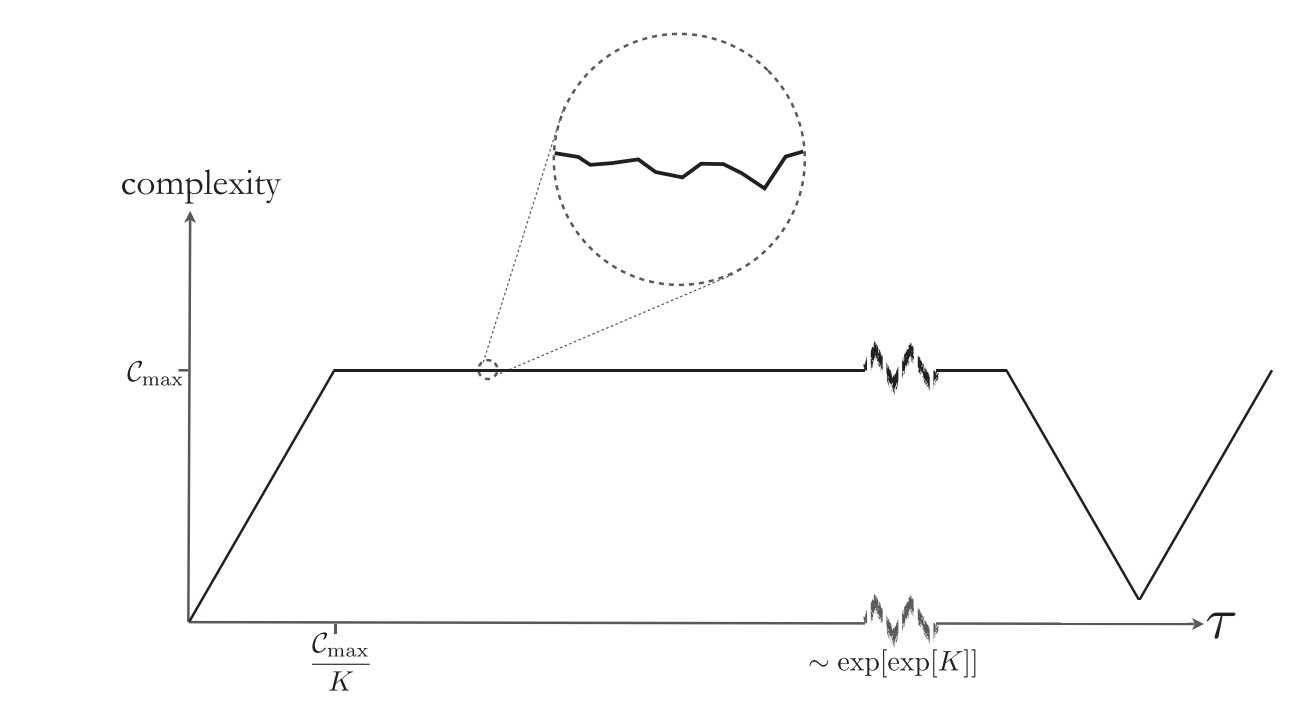
\includegraphics[width=1.1\linewidth]{com_growth.png}
  \caption{The evolution of quantum complexity with time.}
 \end{minipage}\hfill
 \begin{minipage}{0.45\linewidth}
  \centering
  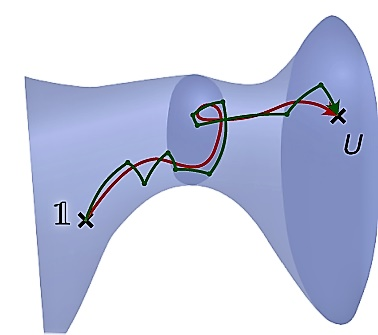
\includegraphics[width=0.8\linewidth]{space.jpg}
  \caption{The green path represents the evolution of a discrete circuit, and the red path represents Hamiltonian evolution. The quantum complexity is the shortest path from $\mathbb{1}$ to $\textit{U}$.}
 \end{minipage}
 
\end{figure}
Moreover, a counting argument that uses graph theory to describe circuits \cite{brown2018second} showed that the number of unitaries of complexity $\mathcal{C}$ grows exponentially with $\mathcal{C}$. In other words, the volume of SU($2^K$) grows exponentially with $\mathcal{C}$. This supports the conjecture that the quantum complexity is directly related to entropy, since in classical statistical mechanics, the volume of the phase space associated with an ensemble of states of a given entropy grows exponentially with the entropy.

\section{The second law of quantum complexity}
This deep analogy between complexity and entropy in a classical chaotic system suggests that a second law of complexity can be defined. Therefore, the second law of quantum complexity \cite{brown2018second} is: 
\begin{adjustwidth}{0.5cm}{0pt}
 ``If the computational complexity is less than maximum, then with overwhelming likelihood it will increase, both into the future and into the past.''
\end{adjustwidth}
Thus we can understand the growth of quantum complexity of a K-qubit system by studying the evolution of classical entropy of an auxiliary system of $2^K$ degrees of freedom.
\\
In principal, we can prepare a quantum system that evolves toward decreasing complexity by inverting the sign of the Hamiltonian. In classical physics, inverting the trajectory in phase space leads to a decrease in entropy. However, this violation of the second law of thermodynamics is unstable when the system is chaotic, since a change in a single degree of freedom grows exponentially and quickly reverses this decrease. Therefore, the quantum-classical duality between the quantum system and the auxiliary one implies that a small perturbation in the form of a single qubit reverses the compleixty decrease.
\\
\\
Although the quantum complexity of $\mathcal{Q}$ is analogous to the classical entropy of the auxiliary system $\mathcal{A}$, we should not confuse the entropy of $\mathcal{A}$ and the actual entropy of $\mathcal{Q}$. The entropy of $\mathcal{Q}$ will only increase for a polynomial time in the number of qubits before $\mathcal{Q}$ comes to thermal equilibrium. However, the complexity of $\mathcal{Q}$ continues to grow long after thermal equilibrium is attained. 

\section{Uncomplexity and the power of one ``clean qubit"}
In classical thermodynamics, the way to quantify how much mechanical work can be extracted from an amount of energy is to measure the negentropy. Negentropy is the difference between the maximum entropy that a system can attain ($S_{max}$) and the system’s actual entropy (S). If the negentropy is not zero, then we can extract a certain amount of work from the system by expending some of the negentropy. When all the negentropy is expended, the system will have reached thermal equilibrium, and no more work can be extracted.
\\
Motivated by the analogy between the quantum complexity of $\mathcal{Q}$ and the classical entropy of $\mathcal{A}$, Brown and Susskind \cite{brown2018second} defined “uncomplexity” as the gap between the actual complexity and the maximum possible complexity of the system:

\begin{center}
Uncomplexity $ \equiv \Delta \mathcal{C} = \mathcal{C}_{max} - \mathcal{C} $
\end{center}

Similar to the negentropy, uncomplexity is a resource for doing some kind of work, which is in this case directed computational work, i.e. computation with a goal.
\\
If the state of the system has reached maximal complexity, exponential in the number of qubits, then $ \Delta \mathcal{C} = 0 $, and the state is useless for computations. Conversely, a simple unentangled prodcut state has $\mathcal{C}$ = 0, which means it is the most powerful initial state for a general computation.
\\
\\
In thermodynamics, it is important to understand how to combine two isolated systems which are both in thermal equilibrium. Therefore, it is essential that we understand how to combine two auxiliary systems and their corresponding quantum systems.
\\
We might think that combining two auxiliary systems $\mathcal{A} \times \mathcal{A} $ that are in thermal equilibrium involves combining the two corresponding quantum systems that are in complexity equilibrium in the form $ \mathcal{Q} \otimes \mathcal{Q}$. However, if each subsystem $\mathcal{Q}$ contains K qubits, then it has complexity $ \sim 2^K $, and the combined system would have complexity $ \sim 2^{(2K)} $. On the contrary, the total entropy of the auxiliary system would be $ 2 \times 2^K $. This contradicts the conjecture that the quantum complexity is the classical entropy of the auxiliary system. Reference \cite{brown2018second} proves that doubling the quantum system is not doubling the auxiliary system. Evidently, the correct way is to add one single qubit to the quantum system, which results in doubling the dimension of the Hilbert space, and therefore doubling the number of degrees of freedom of the auxiliary system. 
\\
Studying the combination of quantum systems and the addition of one qubit can be used to understand more about how uncomplexity is used as a resource for computational work. For states, the geometry of state complexity is similar to that of unitary operator complexity, but the difference is that SU($2^K$) is replaced by the projective space of normalized states CP($2^K-1$). Consider a maximally complex state in the space of states CP($2^K – 1$). A maximally complex state is mostly indistinguishable from a maximally mixed state if we restrict ourselves to simple nonexponential measurements; the expectation values are Haar random. So no useful computation can result from a maximally complex state. However, by adding a single qubit in a pure state, the maximal complexity doubles while the state’s complexity remains the same. Therefore, the complexity now ($\mathcal{C} = 2^K$) is far from the maximum value ($\mathcal{C}_{max} = 2^{K+1}$), and we can perform useful directed computational work once more. Fig. 3 shows this schematically. Reference \cite{brown2018second} also illustrates an example of how much power adding a clean qubit provides us through computing the trace of a unitary operator in SU($2^K$), which is a classically hard problem. 
 
 %add figure 3
\begin{figure}[h!]
 \begin{framed}
  \centering
  \begin{subfigure}[b]{0.45\linewidth}
   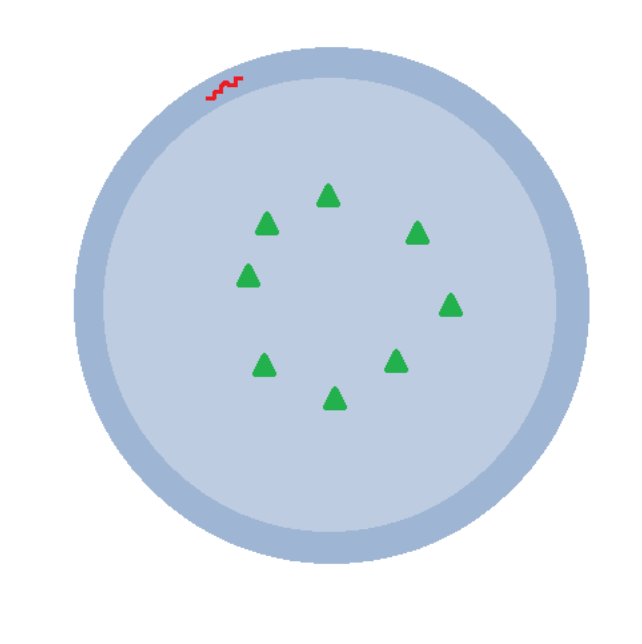
\includegraphics[width=1\linewidth]{max_comp.png}
  \end{subfigure}
  \begin{subfigure}[b]{0.45\linewidth}
   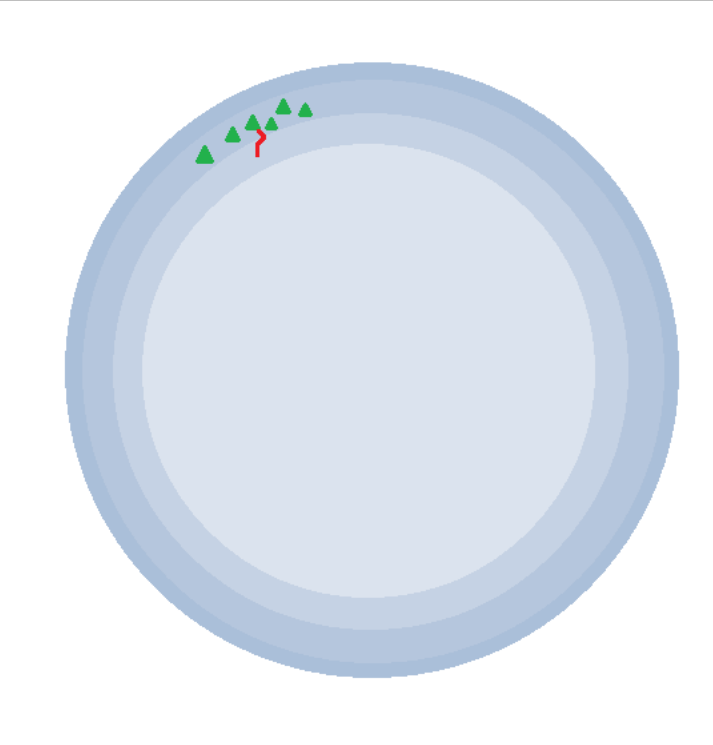
\includegraphics[width=1\linewidth]{double_comp.png}
  \end{subfigure}
  \end{framed}
  \caption{The figure on the left shows a maximally complex state (the red path) is a useless state for computations.
\\
The figure on the right shows the space of states after adding one clean qubit: we can perform computations again.}
\end{figure}
 
\section{Uncomplexity and Spacetime}
The interest in understanding black holes and quantum gravity was the original reason that physicists became interested in complexity. To understand complexity in the context of black holes, we should first understand the following facts.
\\ 
First, after the formation of a black hole, the spatial volume behind the horizon of the black hole continues to grow long past the time when the black hole has come to thermal equilibrium, so it should be related to the complexity.
\\
Consider now a one-sided anti-de Sitter(AdS) black hole. Pick a time t and consider all the co-dimension 1 surfaces anchored to the boundary at time t. The Wheeler-DeWitt(WDW) patch is the union of all those surfaces. This is shown in Fig. 4 (a). It consists of a portion outside the horizon and another one behind the horizon. Moreover, the “complexity equals action” conjecture states that the complexity is given at any instant by the Einstein-Hilbert action of the portion of the WDW patch behind the horizon. This is the darker orange portion in Fig. 4 (a). 
\\
The uncomplexity in this case is the spacetime volume that we can explore if we jump into the black hole after time t. To compute this uncomplexity, we have to know the maximum possible complexity ($\mathcal{C}_{max}$). $\mathcal{C}_{max}$ is shown in Fig. 4(b). Therefore, the uncomplexity is the difference between the maximum complexity and the actual complexity at time t, and it is the blue portion shown in Fig. 4(c). 
\\
In the context of black holes, thermal photons are similar to clean qubits. Suppose the black hole has reached complexity equilibrium, so there is no more spacetime volume to explore inside the black hole. However, for each thermal photon we throw in, the transparency of the horizon is restored for an additional exponential time, similar to how a maximally complex computer can be restored by adding a single clean qubit.

% add fig 4
\begin{figure}[h!]
 \centering
 \begin{subfigure}[b]{0.2\linewidth}
  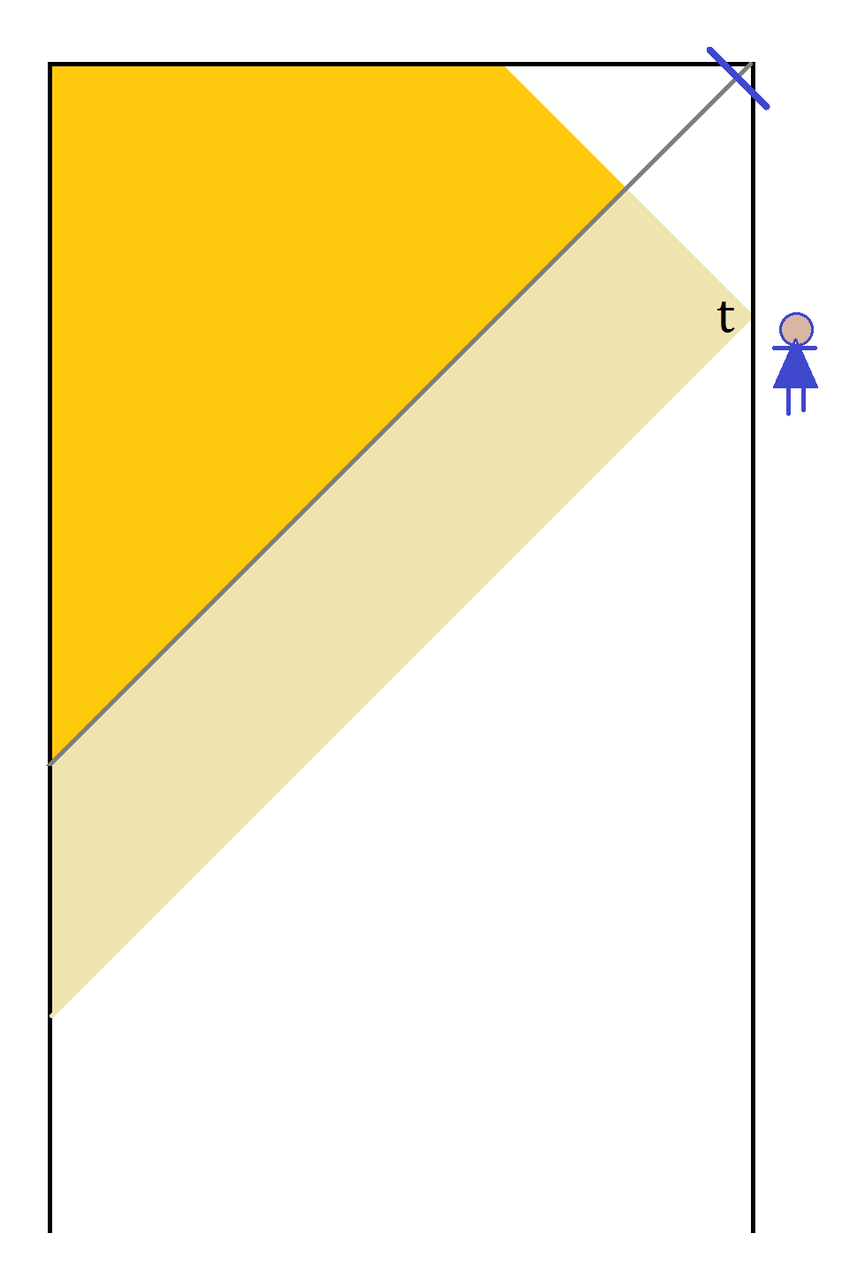
\includegraphics[width=1\linewidth]{penrose_complexity.png}
  \caption{The dark orange region is the complexity at time t.}
 \end{subfigure}
 \begin{subfigure}[b]{0.2\linewidth}
  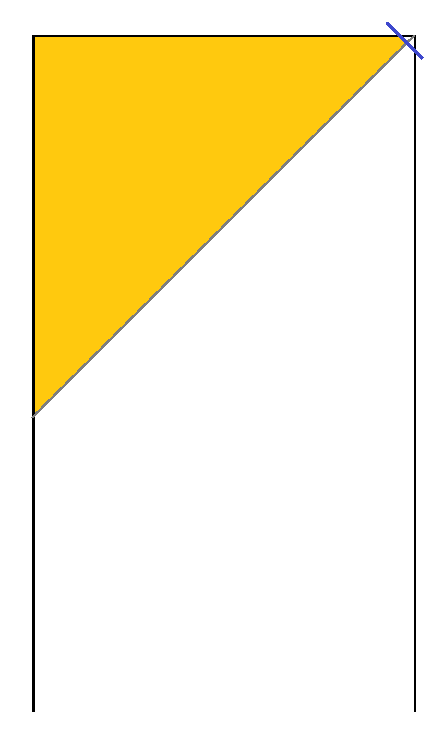
\includegraphics[width=1\linewidth]{penrose_maximum_complexity.png}
  \caption{The dark orange region is the maximum possible complexity.}
 \end{subfigure}
 \begin{subfigure}[b]{0.2\linewidth}
   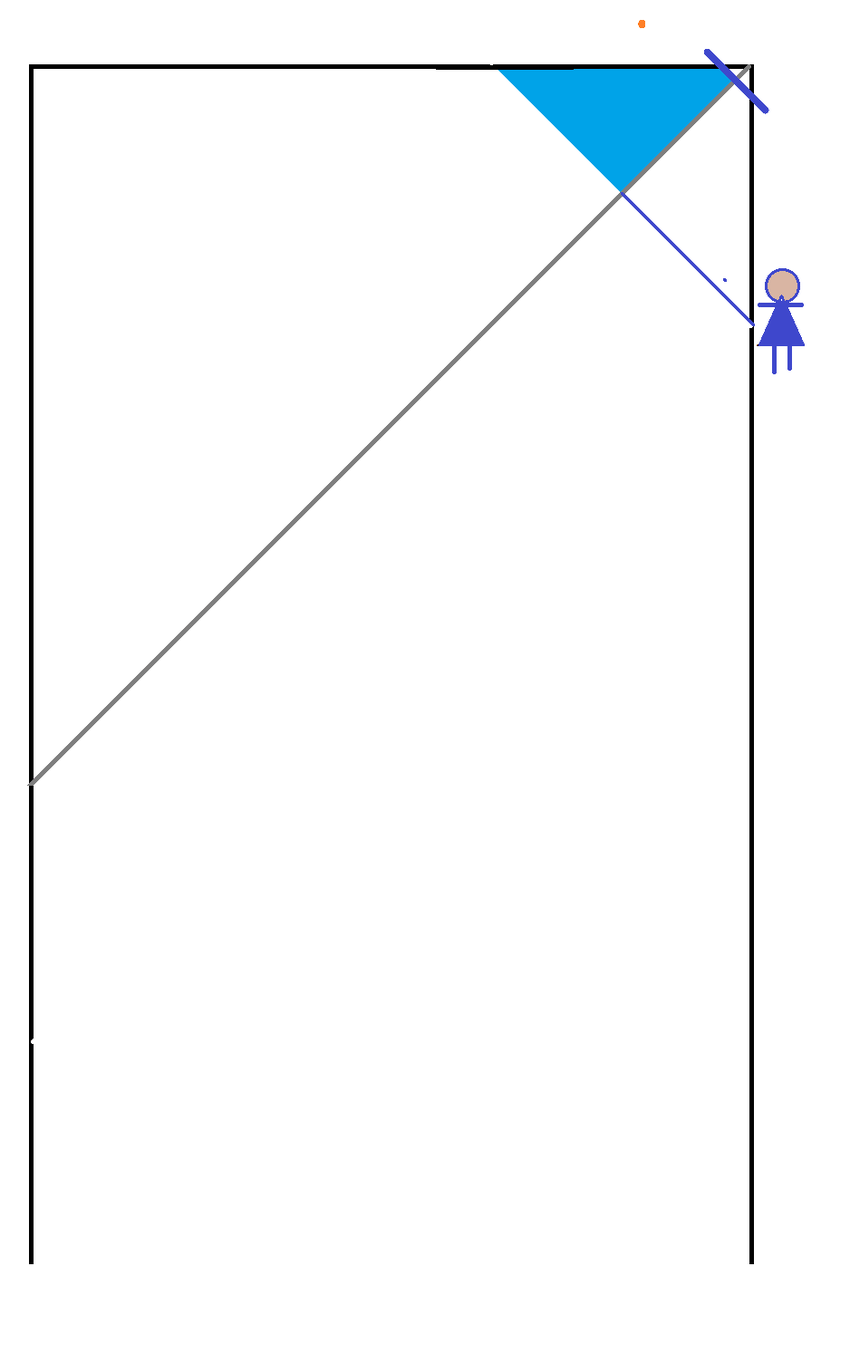
\includegraphics[width=1\linewidth]{penrose_uncomplexity.png}
   \caption{The blue region is the uncomplexity which is $\mathcal{C}_max - \mathcal{C}(t)$.}
  \end{subfigure}
  \caption{}
\end{figure}